\newpage


\section{Convolutional Neural Networks (CNNs)}
\label{sec:convolutional-neural-networks-(cnns)}

Convolutional Neural Networks introduce a powerful tool for defining models that perfectly fits image elaboration.
This tool, which gives the name to the networks, is the \textbf{Convolution layer}.

\paragraph{Convolution}
It applies homonymous mathematical operation by combining two functions to produce a third one $(f\ast g)(n) = \sum f(m)g(n-m)$,
where, in the context of images, $f$ could represent an image and $g$ a kernel.

More intuitively the kernel combines the pixels of images in a window, given by its size,
to generate altered values based on the neighborhood.
In neural network this is not any different as the weighted inputs are convoluted by the kernel specification.

In image processing convolution is a basic element for many tasks, and it becomes powerful in neural networks
as the learning process gives values to the kernel matrices.
The power in applying convolutions to the data is that it can alter information contained to better show features of
the image, which is what we often see in shown examples, from simple lines to complex shapes the deeper the convolutions.

In keras this is obtained by the \textbf{Conv2D}\cite{con2d} layer object, such as:
\begin{verbatim}
x = keras.layers.Conv2D(
    filters=64, kernel_size=(3,3), padding="same", activation="relu"
)
\end{verbatim}

\paragraph{Pooling}
The convolution layer provided in most machine learning frameworks can be configured in a way that the layer produces
smaller data from one layer to the following in order to reduce the amount of parameters and computations required by the network.

In the project, this functionality was provided in a further dedicated \textbf{Pooling} layer.
The pooling operation simply down-samples the feature map of the data. In keras this is achived by any implementation
of the pooling operation. As the difference between different techniques doesn't lead to a satisfing
conlcusion\cite{bieder2021comparison}, the \textbf{MaxPooling2D}\cite{maxpooling2d} was used as it is the go to for starters:


\begin{verbatim}
# The pool_size defines the windows on which max-pooling is applied.
# Stride is by default set to None and not used.
x = keras.layers.MaxPooling(pool_size=(2,2))
\end{verbatim}




For a long time CNN have been the state of the art for various fields involving machine learning, including Computer Vision.
Now that transformers have become popular CNN might have been outclassed but the question is still open for debate.\cite{wang2023cnns}
Besides being very effective the fact that they are both easier to train and less memory constraining were other good reasons
to favor CNNs instead of the simple MLPs approach.

\subsection{Model Structure}
% todo finish with images
\paragraph{First Model}

\begin{figure}[h]
    \centering
    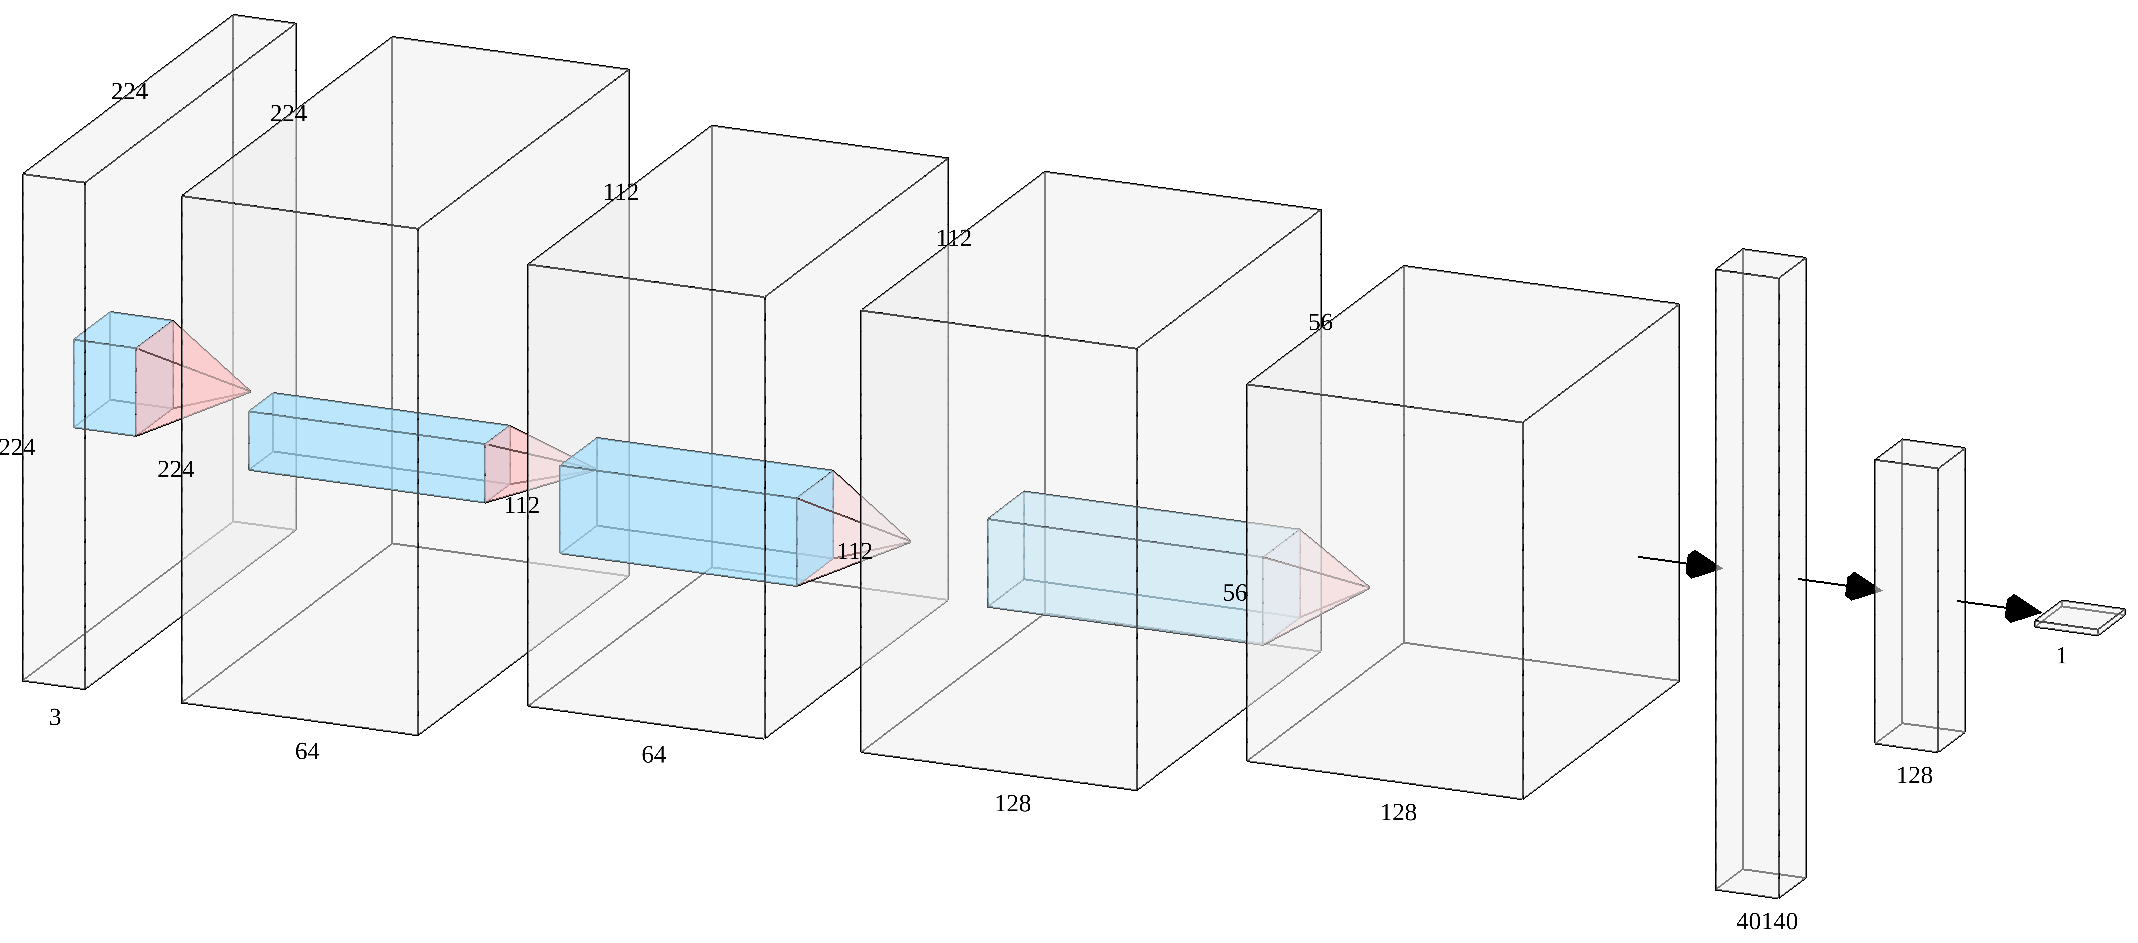
\includegraphics[scale=0.15]{imgs/custom-cnn-one}
    \caption{
        Graphical representation of the first CNN model. (Not in scale)\\
        \textit{Image generated via the NN-SVG tool}
    }\label{fig:custom_cnn}
\end{figure}



\paragraph{Second Model}

\begin{figure}
    \centering
    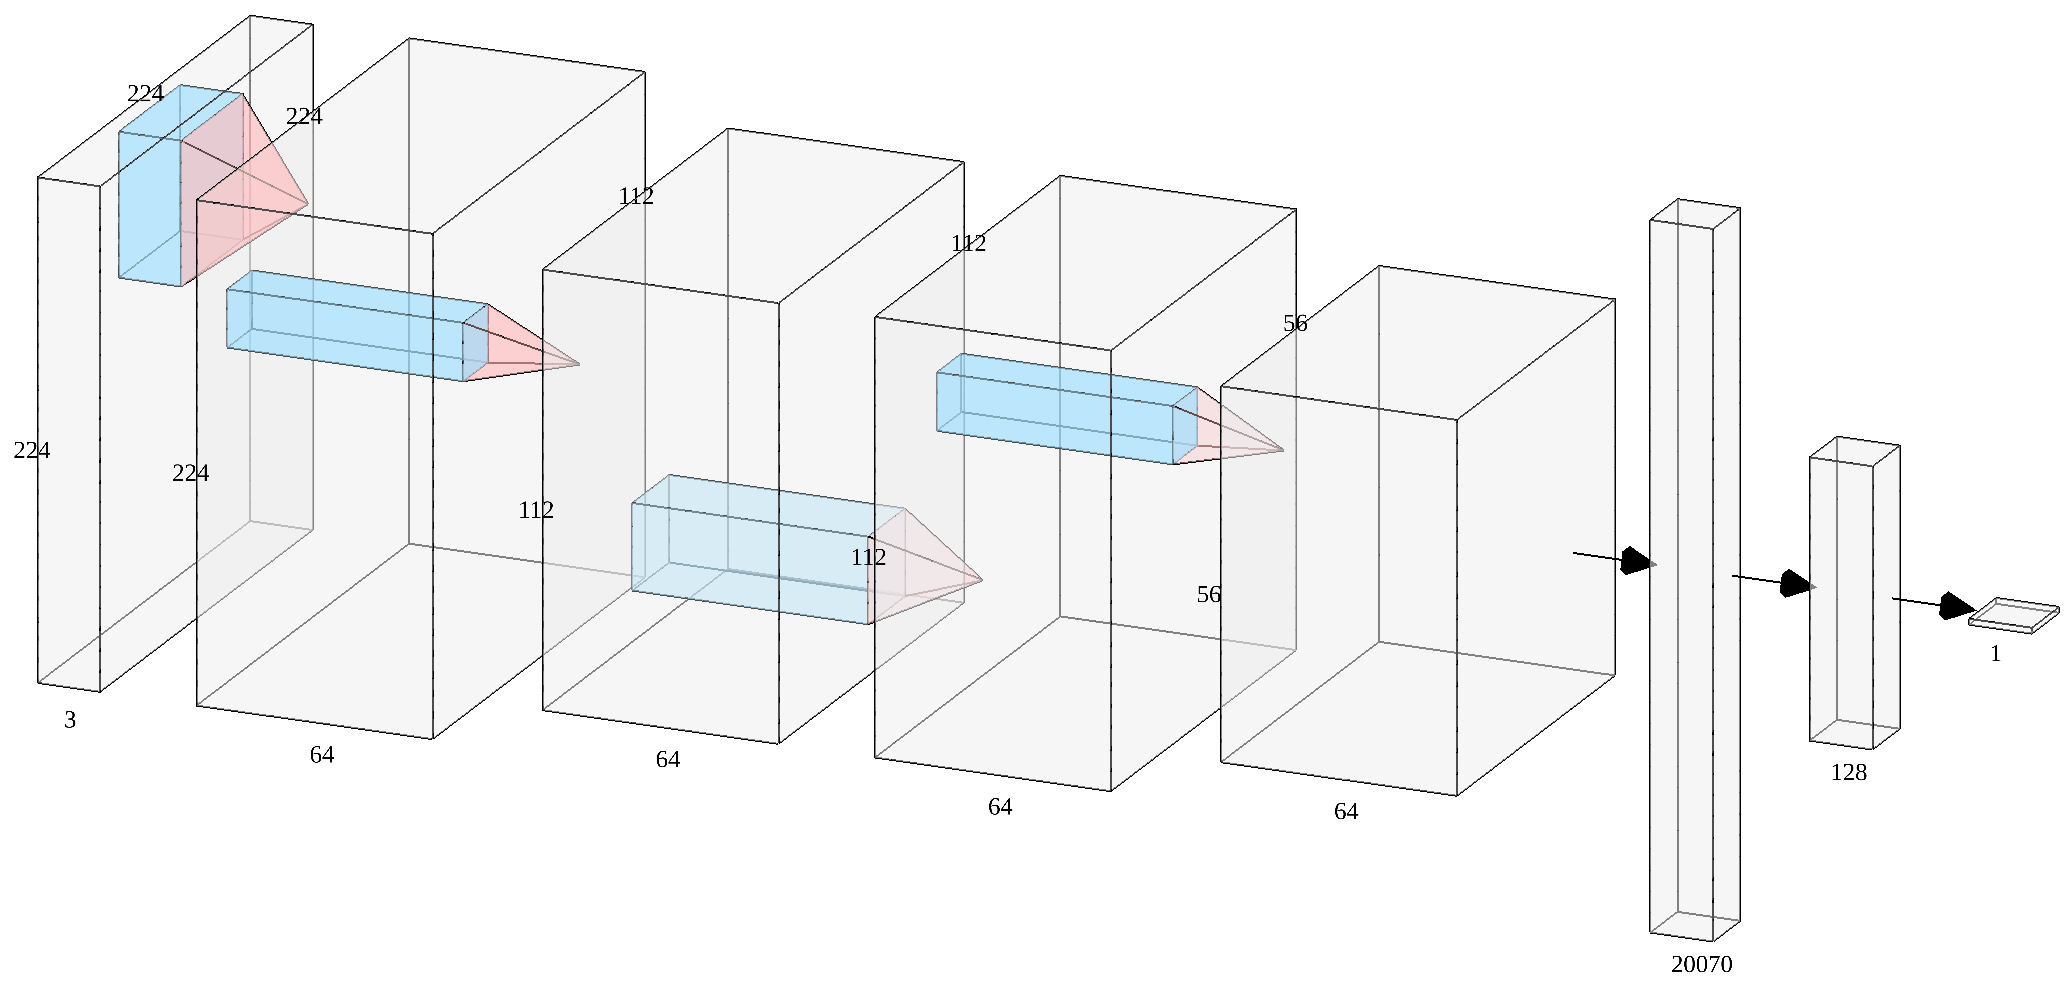
\includegraphics[scale=0.15]{/home/jacopo/PycharmProjects/muffin-stat-project/report/imgs/second-conv-net-structure}
    \caption{
        Graphical representation of the second CNN model. (Not in scale)\\
        \textit{Image generated via the NN-SVG tool}
    }
    \label{fig:second-conv-net-structure}
\end{figure}

\subsubsection{Autotuned CNN}
While the CNN yield not bad results given their simplicity a better structure could be sure identified.
Instead of going on by trial and error we wanted to auto-tune the architecture of the network itself.

In order to do this, and testing a good amount of combinations, the search space was confined to:
\begin{description}
    \item [convolutional\_layers] The amount of $(CONV \rightarrow POOL)$ layers to build.\\
    For each of these, the pooling layer parameters were fixed.
    \item[filters\_i] Number of specified filters, a power of two from 16 to 256, for the convolution layer $i$
    \item[kernel\_i] The square size of the kernel chosen from the set of values: ${3,5}$ for the convolution layer $i$
    \item[hidden\_layers] Number of dense layers that follow the convolutional ones
    \item[units\_i] Number of units for the dense layer $i$
\end{description}

The optimization process has run for a total of 40 iterations and resulted in various models with a close performance.
From the results it is noticeable that the ones with more convolutional layers generally lead to better results.

\paragraph{Auto-tuned Model}

The best performing model is of the structure:
% struttura del coso

On this model we also fine-tuned the learning parameters. % todo devi spiegare da qualche parte il fine tuning

\subsection{Observed Results}

The k-fold CV estimates are:
% imamgeine estiamtes